% Kompiuterijos katedros ir kibernetinio saugumo laboratorijos šablonas
% Template of Department of Computer Science II or cybersecurity laboratory
% Versija 1.4 2024 m. sausi [ March, 2015]
% comments/bug fixes send to template authors: Linas Bukauskas or Agnė Brilingaitė
\documentclass[a4paper,12pt,fleqn]{article}
\usepackage[unicode,colorlinks=false]{hyperref}


\usepackage[utf8x]{inputenc}
%

\usepackage[L7x]{fontenc}
\usepackage{times}
\usepackage{ucs}
%\usepackage{microtype}
%\DisableLigatures{encoding = *, family = *}
 %package to switch the language
\usepackage{etoolbox}

  %set up of the page margins
\usepackage[top=2cm, bottom=2cm, left=3cm, right=1.5cm]{geometry}

 %1.1 line spacing
\linespread{1.1}


  %page numbering at the right side
\usepackage{fancyhdr}
\pagestyle{fancyplain}
\fancyhf{}
\renewcommand{\headrulewidth}{0pt} 
\fancyhfoffset[RO]{0cm}

  %to number at the bottom (exchange lines to number at the top)
\rfoot{\thepage}
  %\rhead{\thepage} %

% \usepackage[usenames,dvipsnames]{pstricks}
\urlstyle{same}
\hypersetup{
%  citecolor=Blue,
%  linkcolor=Blue,
%  urlcolor=Blue
pdfborder={0 0 0 }
}

 %for includegraphics
\usepackage{graphicx}

\usepackage[toc,page]{appendix}


\usepackage{caption}

 %for source codes
\usepackage{listings}
\lstset{commentstyle=\color{red},xleftmargin=10pt, framexleftmargin=6pt, numbersep=1mm, frame=single, numbers=left,numberstyle=\footnotesize,extendedchars=\true, inputencoding=utf8x,basicstyle=\footnotesize,extendedchars=true,
 keywordstyle=\color{black}\bfseries, breaklines=true, breakautoindent=true,framesep=8pt,linewidth=0.95\textwidth
}

 %for algorithms
\usepackage{algorithm}
\usepackage{algorithmic}
 %instead of the above two packages we can use algorithms2e
 %\usepackage[boxed,linesnumbered,vlined,slide]{algorithm2e}

 %special symbols
\usepackage{amsfonts}
%\usepackage{amssymb} %redundant
\usepackage{amsmath}

 %for theorem like environments
\usepackage{amsthm}

 \usepackage{datetime}
 \renewcommand{\dateseparator}{--}


% SI system units
\usepackage{siunitx}
\sisetup{detect-all}
% Problem with fonts \SI{x.xx}{\micro\metre}, solved with updmap-sys --enable Map=utm.map
\renewcommand{\sfdefault}{uhv}
%\renewcommand{\rmdefault}{utm}  %commented due to text missformating
\usepackage{stix}
\renewcommand{\ttdefault}{ucr}

% List management (itemize, etc.)
\usepackage{enumitem}

\newcommand*{\urlw}[1]{\href{#1}%
            {\nolinkurl{#1}}}

\numberwithin{equation}{section}


%%%%%%%%%%% lino įdėta
%
\usepackage{pifont,mdframed}

\newenvironment{warning}
  {\par\begin{mdframed}[linewidth=2pt,linecolor=red]%
    \begin{list}{}{\leftmargin=1cm
                   \labelwidth=\leftmargin}\item[\Large\ding{43}]}
  {\end{list}\end{mdframed}\par}
  
\usepackage{graphicx}
\newtoggle{inLithuanian}
 %If the report is in Lithuanian, it is set to true; otherwise, change to false
\settoggle{inLithuanian}{false}

%create file preface.tex for the preface text
%if preface is needed set to true
\newtoggle{needPreface}
\settoggle{needPreface}{false}

\newtoggle{signaturesOnTitlePage}
\settoggle{signaturesOnTitlePage}{false}


\theoremstyle{definition}
\newtheorem{definition}{\keyWordDefinition}
\newtheorem{example}{\keyWordExample}
\def\QED{\unskip\nobreak\hfill\kern5pt$\Box$}

\iftoggle{inLithuanian}{
%\usepackage[L7x]{fontenc}
\usepackage[english,lithuanian]{babel}

\newcommand{\todayiso}{\the\year \dateseparator \twodigit\month \dateseparator \twodigit\day}


\renewcommand{\today}{\number\year\space m. \space \ifcase\month\or
  sausio\or vasario\or kovo\or balandžio\or gegužės\or birželio\or
  liepos\or rugpjūčio\or rugsėjo\or spalio\or lapkričio\or
  gruodžio\fi
  \space\number\day\space d.}


 \usepackage{tocloft}
 \renewcommand\cftsecaftersnum{.} 
 \renewcommand\cftsubsecaftersnum{.} 
 \renewcommand\cftsubsubsecaftersnum{.}

 \usepackage{VUMIFKK}

 \DeclareCaptionLabelFormat{captionlt}{#2 #1}
   %smth is not fine with algorithms 
 \DeclareCaptionLabelFormat{captionltalg}{#2 #1 algoritmas}

 \usepackage{indentfirst}
 \renewcommand{\appendixtocname}{Priedai}
 \renewcommand{\appendixpagename}{Priedai}
 \renewcommand{\contentsname}{Turinys} 

 \renewcommand{\lstlistingname}{išeities kodas}
 \renewcommand{\figurename}{pav}
 \renewcommand{\tablename}{lentelė}


 \captionsetup*[lstlisting]{   
 labelsep=period,labelformat=captionlt
 }
 \captionsetup*[figure]{   
% labelsep=period,
 labelsep=space, %babel redefines pav to pav.
 labelformat=captionlt
 }
 \captionsetup*[table]{   
  labelsep=period,
  labelformat=captionlt
 }
 \renewcommand{\algorithmicrequire}{\textbf{Įvestis:}}
 \renewcommand{\algorithmicensure}{\textbf{Išvestis:}}

 \captionsetup*[algorithm]{   
 labelsep=period,labelformat=captionltalg
 }

\renewcommand{\thmhead}[3]{#2 #1#3}

}
{
%\usepackage[OT1,T1]{fontenc}
%\usepackage[L7x]{fontenc}



\usepackage[english]{babel}
\newcommand{\todayiso}{\twodigit\month \dateseparator \twodigit\day \dateseparator \the\year}
 \captionsetup*[algorithm]{   
 labelsep=period
 }
\captionsetup*[lstlisting]{   
 labelsep=period
 }
 \captionsetup*[figure]{   
 labelsep=period
 }
 \captionsetup*[table]{   
 labelsep=period
 }


}

%some kywords
 \def\keywordAbstract{\iftoggle{inLithuanian}{Santrauka}{Abstract}}
 \def\keywordAbstractOther{\iftoggle{inLithuanian}{Summary}{Santrauka}}
 \def\keyWordIntroduction{\iftoggle{inLithuanian}{Įvadas}{Introduction}}
 \def\keyWordConclusions{\iftoggle{inLithuanian}{Išvados ir rekomendacijos}{Conclusions and Recommendations}}

 \def\keyWordPreface{\iftoggle{inLithuanian}{Pratarmė}{Preface}}
 \def\keyWordAppendice{\iftoggle{inLithuanian}{Priedas}{Appendix}}
 \def\keyWordSignature{\iftoggle{inLithuanian}{parašas}{signature}}
 \def\keyWordDefinition{\iftoggle{inLithuanian}{apibrėžimas}{Definition}}
 \def\keyWordExample{\iftoggle{inLithuanian}{pavyzdys}{Example}}

\newcommand{\bothabstracts}[3]{
\setcounter{secnumdepth}{0}
\newpage
\hspace{2cm}
{\centering{\section{\keywordAbstract}}}

#1
\newpage
\hspace{2cm}
{\centering \section{\keywordAbstractOther}}

\begin{center}{\textbf{#2} }\end{center}

 #3
\setcounter{secnumdepth}{3}
}

 %non-numbered sections: #1 param: for labeling sec:#1, #2 -section title
\newcommand{\sectionWithoutNumber}[2]{\newpage
%\hspace{2cm}
\section*{#1}
\label{sec:#2}
\addcontentsline{toc}{section}{\nameref{sec:#2}}%{#3}
 }



\newcommand{\referenceSources}[1]{
\newpage
\cleardoublepage
\phantomsection
\iftoggle{inLithuanian}{
 \renewcommand{\refname}{Literatūros šaltiniai}

 \addcontentsline{toc}{section}{Literatūros šaltiniai}
 \markboth{\refname}{Literatūros šaltiniai}
 }
{

\addcontentsline{toc}{section}{References}
\markboth{References}{References}
}

\bibliographystyle{plain}
\bibliography{#1}
}



 \newcommand\authorsignature[1]{
\begin{flushright}
 \begin{minipage}[b]{0.45\textwidth}
  \centering
  \rule{\textwidth}{0.5pt}\\
   #1
  \end{minipage}
\end{flushright}
 }




 \newcommand\authorsignatures[5]{%
   \vspace{1cm}
   \authorsignature{#1}
   \ifstrequal{#2}{}{}{\vspace{0.3cm}
     \authorsignature{#2}
     \ifstrequal{#3}{}{}{\vspace{0.3cm}
      \authorsignature{#3}
      \ifstrequal{#4}{}{}{\vspace{0.3cm}
        \authorsignature{#4}
        \ifstrequal{#5}{}{}{\vspace{0.3cm}
         \authorsignature{#5}       
        }
      }
    }
} 
}

\newcommand{\authortitle}{
\iftoggle{signaturesOnTitlePage}{
\tiny{\keyWordSignature}
}{}
}

\newcommand{\depttitlepage}[8]
{
\thispagestyle{empty}
\begin{center}


\includegraphics[width=2cm]{jb_VU_zenklas}

%\vspace{-1cm}

\iftoggle{inLithuanian}
{ 
  VILNIAUS UNIVERSITETAS\\
  MATEMATIKOS IR INFORMATIKOS FAKULTETAS\\
  INFORMATIKOS INSTITUTAS\\
  <<KOMPIUTERINIO IR DUOMENŲ MODELIAVIMO KATEDRA>> ARBA \\ <<KIBERNETINIO SAUGUMO LABORATORIJA>>
}
{
  VILNIUS UNIVERSITY \\
  FACULTY OF MATHEMATICS AND INFORMATICS \\
  INSTITUTE OF COMPUTER SCIENCE\\
  <<DEPARTMENT OF COMPUTATIONAL AND DATA MODELING>> OR \\ <<CYBERSECURITY LABORATORY>>
}

\vspace{5cm}

#1\\
\vspace{0.5cm}
\textbf{\Large #2}
\end{center}

\vspace{5cm}


\hspace{0.5\textwidth}
\begin{minipage}{0.4\textwidth}
 \begin{flushleft} 
\iftoggle{inLithuanian}
{
 \ifstrequal{#3}{}{}{Atliko:\\[5pt]}
}
{
\ifstrequal{#3}{}{}{Done by:\\[5pt]}
}
%\noindent
\begin{tabular}{@{}lr}%\setlength\tabcolsep{0pt}
\ifstrequal{#3}{}{}{#3&\hspace{2cm}\authortitle\\[5pt]}
\ifstrequal{#4}{}{}{#4&\authortitle\\[5pt]}
\ifstrequal{#5}{}{}{#5&\authortitle\\[5pt]}
\ifstrequal{#6}{}{}{#6&\authortitle\\[5pt]}
\ifstrequal{#7}{}{}{#7&\authortitle\\}
\end{tabular}

\end{flushleft}

\end{minipage}

\vspace{0.5cm}
\hspace{0.5\textwidth}
\begin{minipage}{0.4\textwidth}
 \begin{flushleft} 

\ifstrequal{#8}{}{}
{

\iftoggle{inLithuanian}
{
Vadovas:
}
{
Supervisor:
}

#8

}

\end{flushleft}

\end{minipage}


\vfill

\begin{center}
Vilnius\\
\the\year
\end{center}

\iftoggle{needPreface}{
 \sectionWithoutNumber{\keyWordPreface}{preface}
Pratarmės (Preface) informacija


\iftoggle{inLithuanian}
{
\vspace{\baselineskip}\hfill
\today
}
{
 \vspace{\baselineskip}\hfill \today
}

 \vspace{5cm}

\iftoggle{signaturesOnTitlePage}{}
{
\authorsignatures{#3}{#4}{#5}{#6}{#7}
}
}{}
\newpage
}


\begin{document}
 % #1 -report type, #2 - title, #3-7 students, #8 - supervisor
 \depttitlepage{<<Super programos>> <<x>> kurso <<Darbo/ataskaitos tipas>>}{Darbo pavadinimas rašomąja kalba\\{\small Pavadinimas kita kalba}}{Vardas Vardaitis} 
 {}{}{}{}% students 2-5
{dr. Vadovas Vadovaitis}

\tableofcontents
\newpage


\section{Introduction}

\hspace{1em} The task of this project is to implement, analyse and compare moving average algorithms. Two algorithms
are in the scope of the project: Weighted Moving average (WMA) and Exponential Moving Average (EMA). The
algorithms will be implemented in Python programming language, using NumPy, Pandas, Matplotlib libraries. The
programming will be done in Jupyter Notebook environment. The algorithms will be tested on the same dataset.


\section{Definition of algorithms and signal}

\subsection{Moving Average algorithm}\label{MA}
\hspace{1em} A moving average algorithm is a statistical technique used to analyze sequential data points by creating 
a series of averages of different subsets of the full dataset. Typically applied in time-series analysis, 
finance, and signal processing, it smooths out fluctuations to reveal underlying trends or patterns. 
The algorithm involves calculating the mean of a specified number of data points within a sliding window,
which moves along the dataset, updating the average at each step. This process effectively filters out 
short-term fluctuations, making it easier to identify longer-term trends or patterns within the data.

Given that we have a digital signal \begin{math}
    f_0,f_1,...,f_N
\end{math} and chosen the window size \begin{math}
    K
    \end{math} - positive integer. By applying the moving average algorithm to \begin{math}
        f_i
    \end{math} we get the sum of averages in window of size \begin{math}
        K
    \end{math} to both side. The formula for moving average is:
    \begin{gather}\label{MA_equation}
        g_i = \frac{1}{2K+1} \sum_{j=-K}^{K} f_{i+j},\hspace{1 cm}i = K, K+1, ..., N-K
    \end{gather}
   
    To be noted, the first value of signal that has been averaged value is \begin{math}
        f_K
    \end{math} and the last value is \begin{math}
        f_{N-K}
        \end{math}. The moving average algorithm is used to smooth out short-term fluctuations in the data, 
        however during the process the length of the signal is reduced.
        \subsection{Weighted Moving Average algorithm}\label{WMA}
        \hspace{1em} In the subsection \ref{MA} moving average algorithm was introduced. The moving average 
        algorithm is simple, due to the fact that it averages all the values in the window equally as shown 
        in the formula \ref{MA_equation}. However, in some cases it is more beneficial to give more weight to
        the values that are closer to the current value. This is where the weighted moving average algorithm
        comes in. The weighted moving average algorithm is a variation of the moving average algorithm, where
        the values in the window are given different weights. The formula for weighted moving average is:
        \begin{gather}\label{WMA_equation}
            g_i = \frac{1}{2K+1} \sum_{j=-K}^{K} w_j f_{i+j},\hspace{1 cm}i = K, K+1, ..., N-K, \hspace{1 cm} w_j \sum_{j=-K}^K = 1
        \end{gather}


        The weighted moving average algorithm weights can be defined in various ways. The most common way is to
        use the Gaussian function. The Gaussian function is a bell-shaped curve that is symmetric around the mean.
        The Gaussian function is defined as:
        \newpage
        \begin{gather}\label{Gaussian}
            p(x) = \frac{1}{\sqrt{2\pi}}e^{-\frac{x^2}{2}}
        \end{gather}

        Lets say that \begin{math}
            f_{i-K}
        \end{math} and \begin{math}
            f_{i+K}
        \end{math} 
        should be \begin{math}
            L
        \end{math} times less important than the center value \begin{math}
            f_i
        \end{math}. In this case \begin{math}
            L > 1
        \end{math} is a positive integer, a parameter to weighted moving
        average algorithm. The range of weights distribution could be 
        discretised in range: \begin{math}
            -x_k \leq x \leq x_k
        \end{math}, then it can be calculated where \begin{math}
            x_k \end{math}, is less than center value \begin{math}
                x_0 \end{math} in Gaussian distribution formula \ref{Gaussian}:
                \begin{gather}\label{Gaussian_discretised}
                    \frac{p(0)}{p(x_k)} = L, 
                    \hspace{1 cm} x_k = \sqrt{-2\ln{L}}
                \end{gather}


        To comply with the rule that weights \begin{math}
            \sum_{j=-K}^K w_j = 1
        \end{math} the weights should be normalized. The normalized weights are defined as:
        \begin{gather}\label{Normalized_weights}
            w_j = \frac{p(j)}{\sum_{j=-K}^K p(j)}, \hspace{1 cm} j = -K, -K+1, ..., K
        \end{gather}
        \begin{figure}[ht]
            \centering
            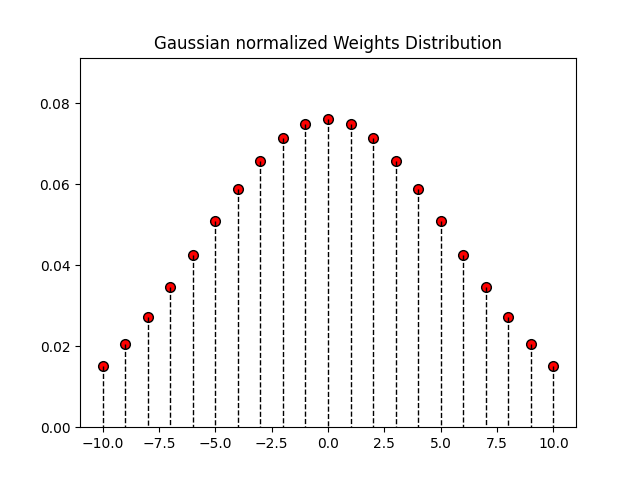
\includegraphics[width=0.8\textwidth]{images/weights.png} % Replace "path/to/your/image" with the actual path to your image file
            \caption{Distribution of normalized weights where L = 10 and K = 30}
            \label{fig:my_image}
        \end{figure}

        \subsection{Exponential Moving Average algorithm}\label{EMA}
        \hspace{1em} The exponential moving average algorithm is another variation of the moving average algorithm.
        This method is similar to the weighted moving average algorithm \ref{WMA}, 
        but have two main diffrences:
        \begin{enumerate}
            \item Instead of parameters \begin{math}
                K
            \end{math} and \begin{math}
                L
            \end{math} the exponential moving average algorithm has only one parameter \begin{math}
                \alpha
            \end{math}.
            \item When new signal value is appended, it is enough to know 
            the previous average value to calculate the new average value. For refrence, 
            other averaging algorithms need to know all the values in the window.
        \end{enumerate}

        To average the signal with exponential moving average algorithm, 
        the formula is used: \begin{gather}
            g_n = (1-\alpha) g_{n-1} + \alpha f_n, \hspace{1 cm} n = 1, 2, \dots , \hspace{1 cm} g_0 = f_0
        \end{gather}
        
        \subsection{Signal for the algorithm analysis}
        \hspace{1em}For the task of this project, the financial market signal was chosen. The daily values of 
        the S\&P 500 index\cite{SP500} at market close from 2014 to 2024 were used. The signal was chosen because it has
         high volatility and represents the financial market well. 


        \begin{figure}[ht]
            \centering
            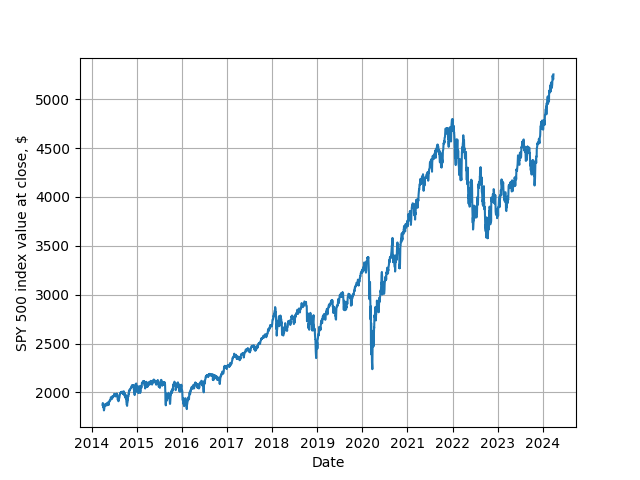
\includegraphics[width=0.8\textwidth]{images/SP500.png} % Replace "path/to/your/image" with the actual path to your image file
            \caption{S\&P 500 index signal from 2014 to 2024}
            \label{fig:SP500}
        \end{figure}

        As can be seen from figure \ref{fig:SP500}, the value of the index have increased over 2.5 times in the
        period of 10 years. The signal has high volatility, which is good for the analysis of moving average algorithms.
        
        For demonstration purposes, these signals will be also used in the project:
        \begin{enumerate}
            \item signal 1
            \item signal 2
            \item signal 3
            \item signal 4
        \end{enumerate}
        
        See the related charts in the section 4 of the assignment.
        \newpage
        \section{Analysis}

        \subsection{Averaging signal with WMA}

        \hspace{1em} The weighted moving average algorithm has two parameters that can be adjusted

        \begin{enumerate}
                \item \begin{math} \bold{K}\end{math} - the size of the window;
                \item \begin{math}
                    \bold{L}
                \end{math} - the parameter that defines the importance of the values in the window.

                \end{enumerate}

                By adjusting these parameters, the algorithm tends to smooth out the signal more or less.
                However, by over tuning the parameters, the algorithm can lose the important information in the signal, i.e.
                the algorithm can over smooth the signal.
                \begin{figure}[ht]
                    \centering
                    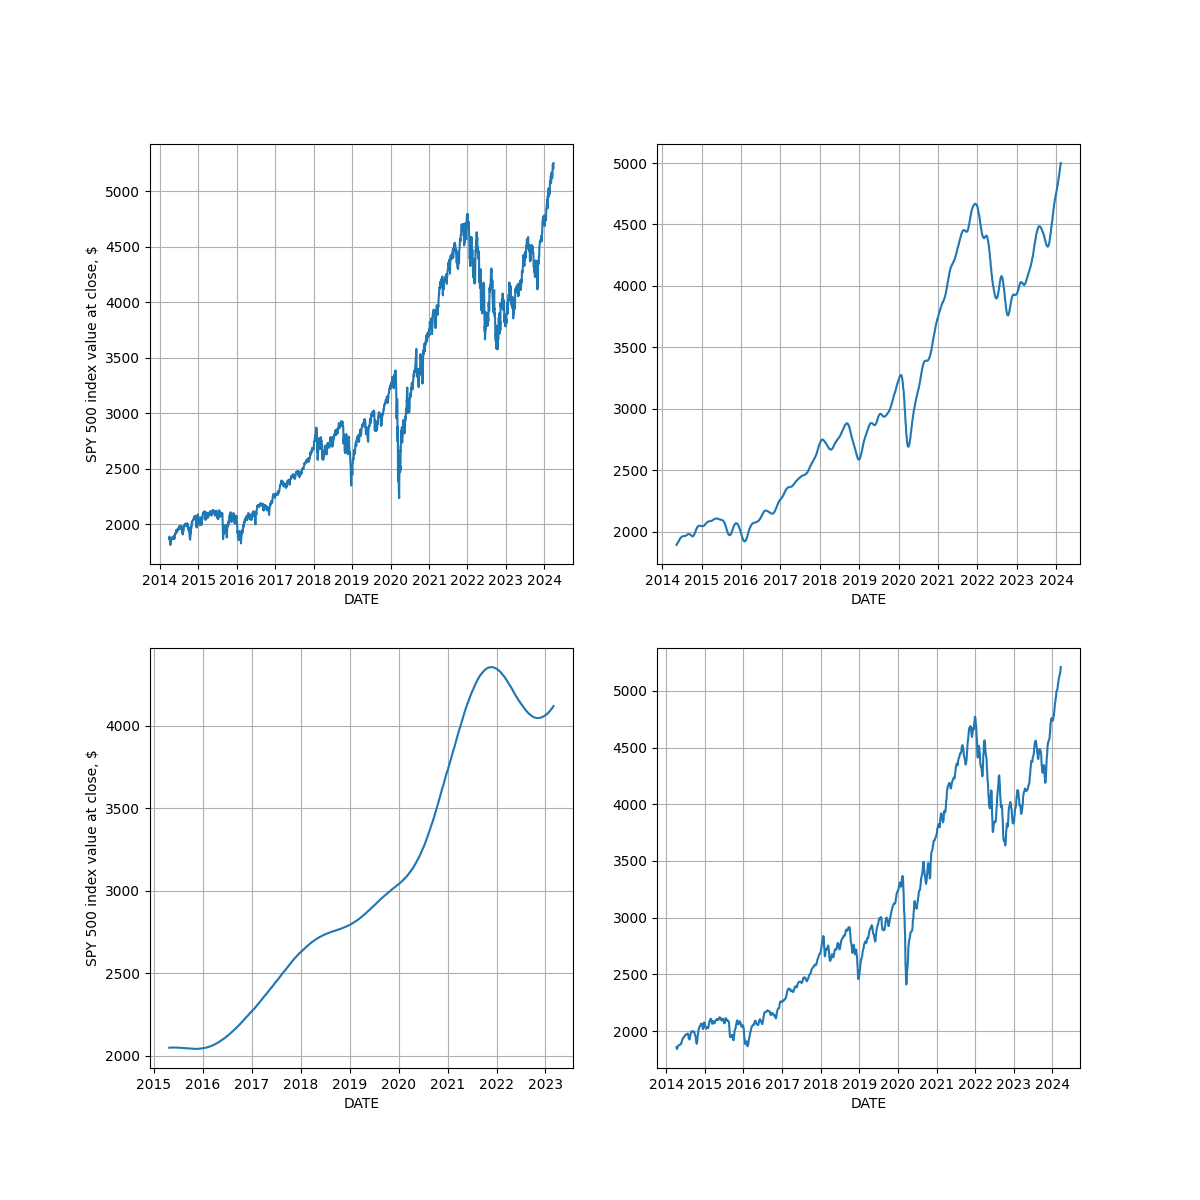
\includegraphics[width=1\textwidth]{images/WMA_ex_1.png} % Replace "path/to/your/image" with the actual path to your image file
                    \caption[Short caption for the list of figures]{On top left chart original signal is shown, on top right chart signal is 
                    averaged with WMA with K = 30 and L = 10, on bottom left chart signal is averaged with WMA  with K = 270 and L = 30, on bottom right chart 
                    signal is averaged with WMA  with K = 5 and L = 5.}
                    \label{fig:WMA_ex_1}
                \end{figure}

                As can be seen from the figure \ref{fig:WMA_ex_1}, the parameters adjust the smoothness of the signal. 
                The larger the \begin{math}
                    K
                \end{math} the smoother the signal gets, also the window of values get shorter,due to 
                algorithms design that only allows to compute values that are in range of
                \begin{math}
                    g = (f_{0+K}; f_{N-K})
                \end{math}
                , see the top left and 
                the bottom left charts in figure \ref*{fig:WMA_ex_1}.
                 The larger the \begin{math}
                    L
                \end{math} the more the values in the window are weighted towards the center value.

                For this particular case study of SP500 signal, the logic parameters for WMA should correlate with the cycles
                of weeks, months, quarters and years. For the case of WMA, parameter \begin{math}
                    K
                \end{math} represents the days that are in window, for example if we set \begin{math}
                    K = 30
                \end{math} the window will be 60 days, which is approximately one month before and one month after to
                the date of intrest.

                \subsection{Qualitative analysis of WMA}

                \hspace{1 em} The main concerns with moving average algorithms 
                is that they tend to lag behind the signal, can be too smooth or retain too much noise. It all depends on
                the parameters that are chosen for the algorithm. The weighted moving average algorithm is more flexible, 
                because it allows to adjust the weights of the values in the window.

                There some methods to evaluate the quality of the algorithm:
                \begin{enumerate}
                    \item Visual inspection of the signal;
                    \item Comparison of the averaged signal with the original signal;
                    \item Evaluating the correlation between the original signal and the averaged signal;
                    \item Evaluating the gradient variance and covariance of the original signal and the averaged signal.
                \end{enumerate}
                \begin{figure}[ht]
                    \centering
                    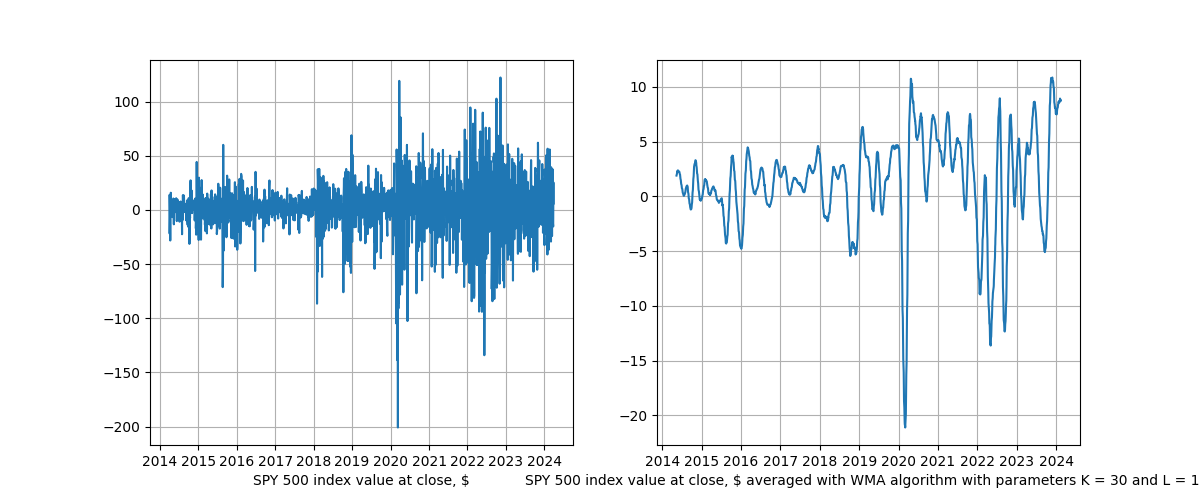
\includegraphics[width=1\textwidth]{images/WMA_ex_2.png} % Replace "path/to/your/image" with the actual path to your image file
                    \caption{In top chart the variance of original signal is shown with variance of = 566.397,
                    in the bottom chart the variance of signal averaged with WMA with K = 30 and L = 10 is shown with variance of = 19.677.}
                \label{fig:WMA_ex_2}
                \end{figure}

                As depicted in figure \ref{fig:WMA_ex_2}, the variance of the signal is reduced by the weighted moving average algorithm.
                The gradient of the signal variance, can help to evaluate if the smoothness of the signal fits the requirements.
                The gradient of the variance can be calculated as:
                \begin{gather}
                    \Delta f = \frac{f_{n+1} - f_n}{f_n}
                \end{gather}

                To evaluate if the averaged signal retains the trends, the correlation between the original signal and the averaged signal 
                can be calculated. The correlation can be calculated as:
                \begin{gather}
                    \rho = \frac{cov(f,g)}{\sqrt{var(f)var(g)}}
                \end{gather}

                \begin{table}[ht]
                    \centering
                    \begin{tabular}{|c|c|c|c|c|c|}
                        \hline
                        & \textbf{K=7} & \textbf{K=30} & \textbf{K=90} & \textbf{K=180} & \textbf{K=360} \\
                        \hline
                        \textbf{L=1} &0.951&0.814 &0.583 &0.391 &0.209 \\
                        \hline
                        \textbf{L=5} &0.951 &0.815 &0.583&0.395 &0.221\\
                        \hline
                        \textbf{L=10} &0.951 &0.815 &0.583&0.396 &0.224 \\
                        \hline
                        \textbf{L=20} &0.951 &0.815 &0.583&0.397&0.227 \\
                        \hline
                        \textbf{L=30} &0.951 &0.816 &0.583& 0.397&0.229 \\
                        \hline
                        \textbf{L=50} &0.951 &0.816 &0.584 &0.398 &0.231 \\
                        \hline
                    \end{tabular}
                    \caption{Matrix of WMA parameters K and L impact on correlation}
                    \label{tab:KL_values}
                \end{table}

                As could be seen from the table \ref{tab:KL_values}, the correlation between the original signal and the averaged signal
                is dependant on the parameter \begin{math}
                    K
                \end{math}. The parameter \begin{math}
                    L
                    \end{math} has negligible impact on the correlation.

                \begin{figure}[ht]
                    \centering
                    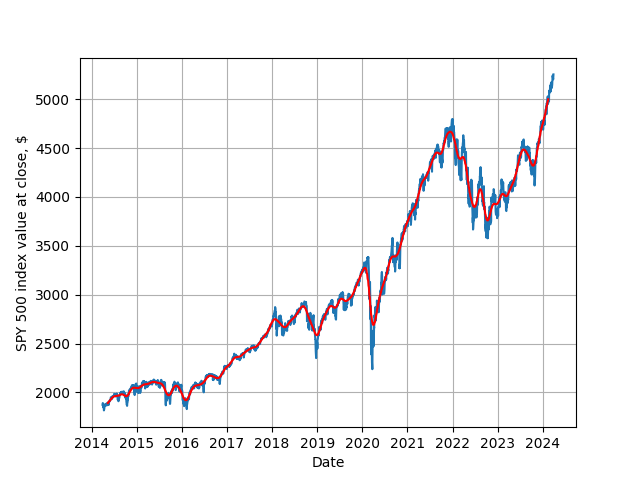
\includegraphics[width=1\textwidth]{images/WMA_ex_3.png} % Replace "path/to/your/image" with the actual path to your image file
                    \caption{S\&P 500 signal from 2014 to 2024 overlayed with signal averaged with WMA with K = 30 and L = 10}
                    \label{fig:WMA_ex_3}
                \end{figure}
\newpage
                \subsection{Averaging signal with EMA}

                \hspace{1 em} EMA has only one parameter \begin{math}
                    \alpha
                \end{math}, which is the weight of the new value in the signal. However, it retains the same
                issues as WMA - if the weight is not chosen correctly, the algorithm can lag behind the signal, be too smooth or retain too much noise.

                \begin{figure}[ht]
                    \centering
                    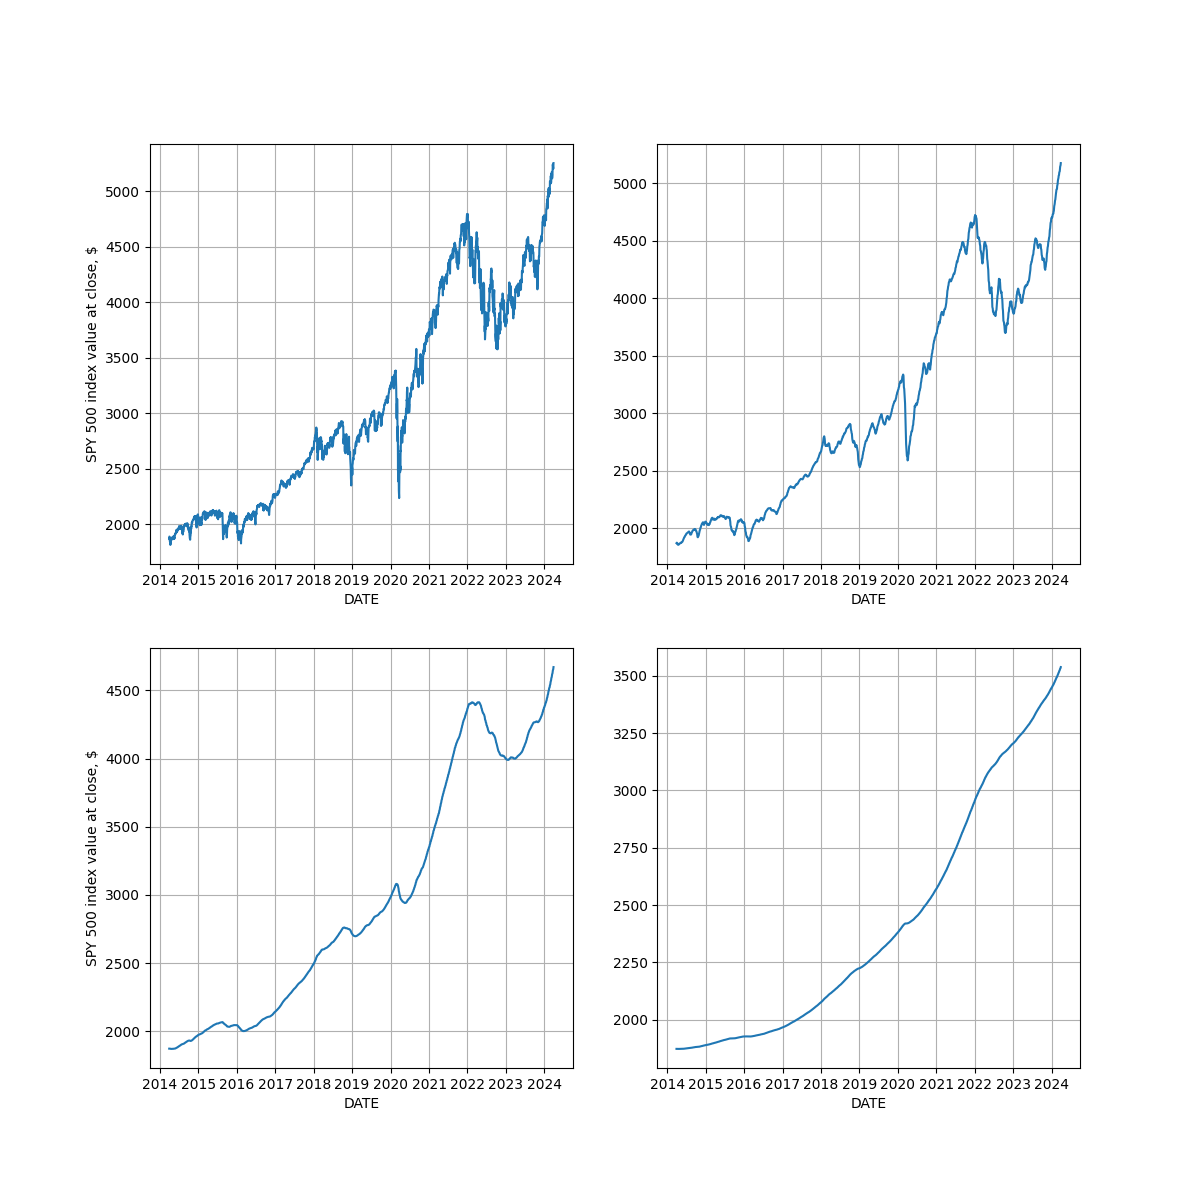
\includegraphics[width=1\textwidth]{images/EMA_ex_1.png} % Replace "path/to/your/image" with the actual path to your image file
                    \caption{On top left chart original signal is shown, on top right chart EMA is applied with $\alpha = 0.1$, on bottom left chart EMA is applied with $\alpha = 0.01$, on bottom right chart EMA is applied with $\alpha = 0.001$.}
                    \label{fig:EMA_ex_1}

                \end{figure}

                As can be seen from the figure \ref{fig:EMA_ex_1}, the smaller the \begin{math}
                    \alpha
                \end{math} the smoother the signal gets and lag occurs.

                Although the EMA algorithm has only one parameter and is more difficult to fine tune, but it has an 
                advantage over the WMA algorithm - it does not require all the values in the window to calculate the new average value. And 
                even next value can be predicted if previous value is known.
                \newpage
                \subsection{Qualitative analysis of EMA}

                The EMA algortithm tends to be more tough for fine tuning, but the same evaluation techniques can
                be adapted for EMA as for WMA. The correlation between the original signal and the averaged signal can be calculated as:
                
                \begin{table}[ht]
                    \centering
                    \begin{tabular}{|c|c|c|}
                        \hline
                        Alpha & Covariance & Correlation \\
                        \hline
                        0.1 & 51.67 & 0.997\\
                        0.08 & 40.53 & 0.996 \\
                        0.06& 29.38 & 0.995 \\
                        0.04& 18.43& 0.993 \\
                        0.02& 8.29 & 0.988 \\
                        0.01& 3.72 & 0.979 \\
                        0.005& 1.50 & 0.967 \\
                        0.001 & 0.22 & 0.944 \\
                       
                        \hline
                    \end{tabular}
                    \caption{Covariance and correlation between original signal and signal averaged with EMA with different $\alpha$ values}
                    \label{tab:correlation_covariance}
                \end{table}
                
            As can be seen from the table \ref{tab:correlation_covariance}, the EMA algorithm tends to retain 
            the trend of the signal better than the WMA algorithm. However, the signal gets smooth in a very short increments of the parameter change.

            \begin{figure}[ht]
                \centering
                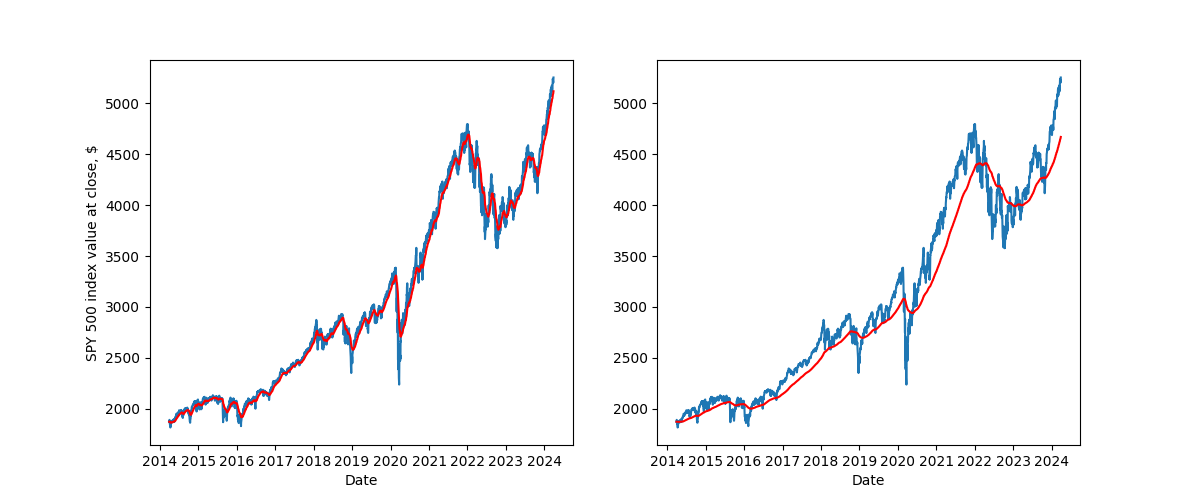
\includegraphics[width=1\textwidth]{images/EMA_ex_2.png} % Replace "path/to/your/image" with the actual path to your image file
                \caption{S\&P 500 signal from 2014 to 2024 overlayed with signal averaged with EMA with $\alpha= 0.06$ on the left side
                and with $\alpha= 0.01$ on the right side.}
                \label{fig:EMA_ex_2}
            \end{figure}

            As can be seen from the figure \ref{fig:EMA_ex_2}, EMA algorithm also tends to lag behind the signal when the
            parameter \begin{math}
                \alpha
                \end{math} is too small.
        \newpage
        \begin{thebibliography}{99}
        \bibitem{SP500} S\&P Dow Jones Indices LLC, S\&P 500 [SP500], retrieved from FRED, Federal Reserve Bank of St. Louis; https://fred.stlouisfed.org/series/SP500, 
        \bibitem{citekey} Author, Title, Year
        \end{thebibliography}
         \end{document}
